\documentclass[a4paper]{article}


%%%%lualatex on
%\usepackage{luatextra}
\usepackage{float}
\usepackage{fontspec}

\begin{document}

%\section{Tournament Size \& Reproductive isolation}

\begin{figure}
    \begin{tabular}[H]{lcccc}
	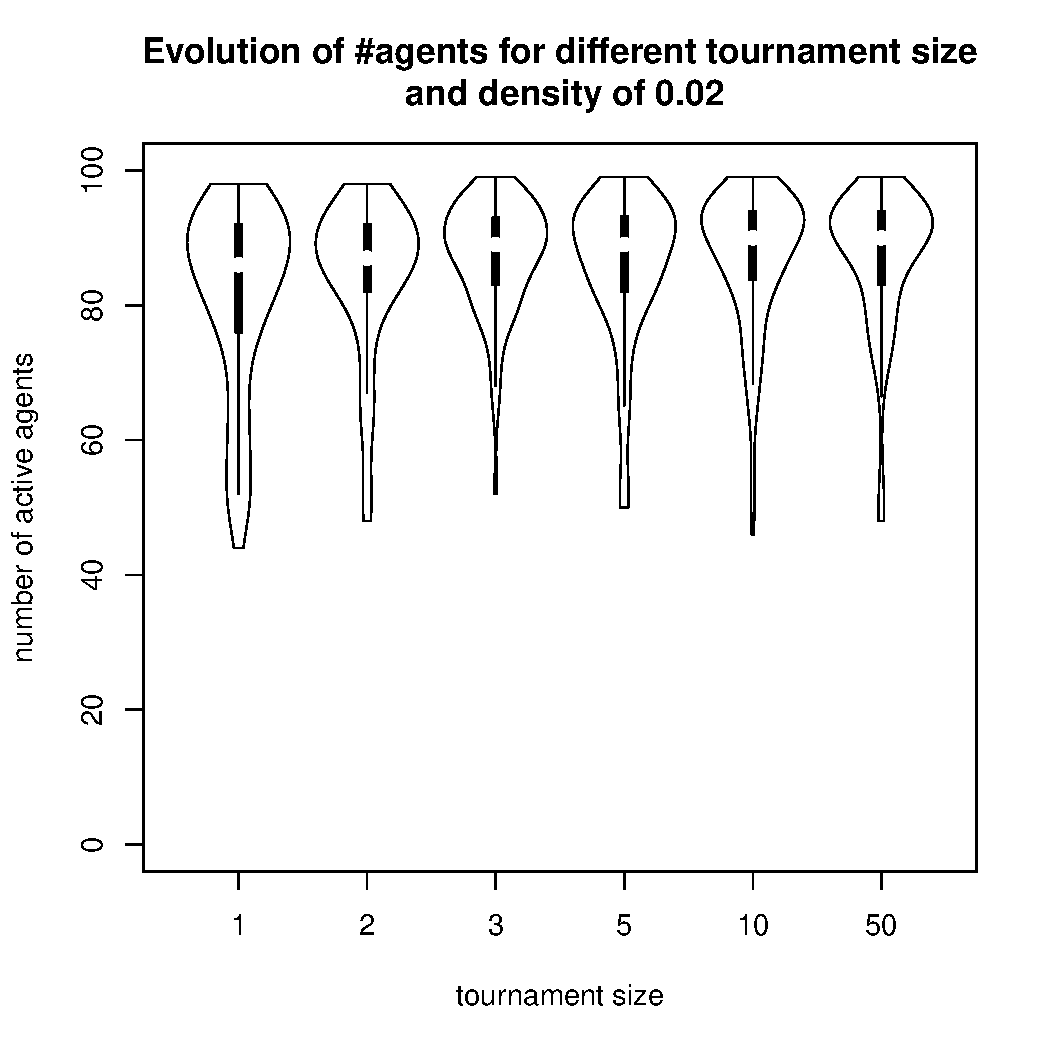
\includegraphics[width=.25\textwidth]{img/100/agentwrtK_D-0020.pdf} &
	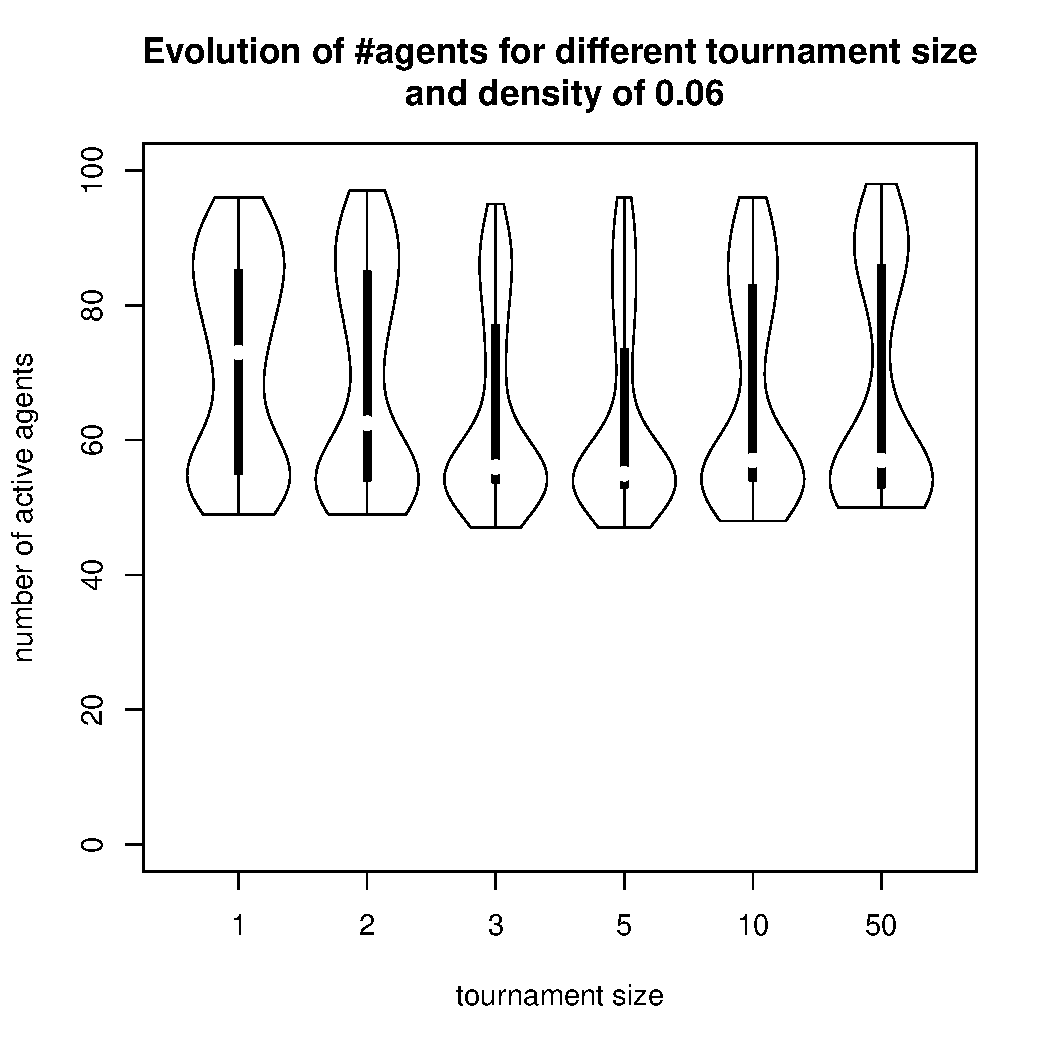
\includegraphics[width=.25\textwidth]{img/100/agentwrtK_D-0060.pdf} &
	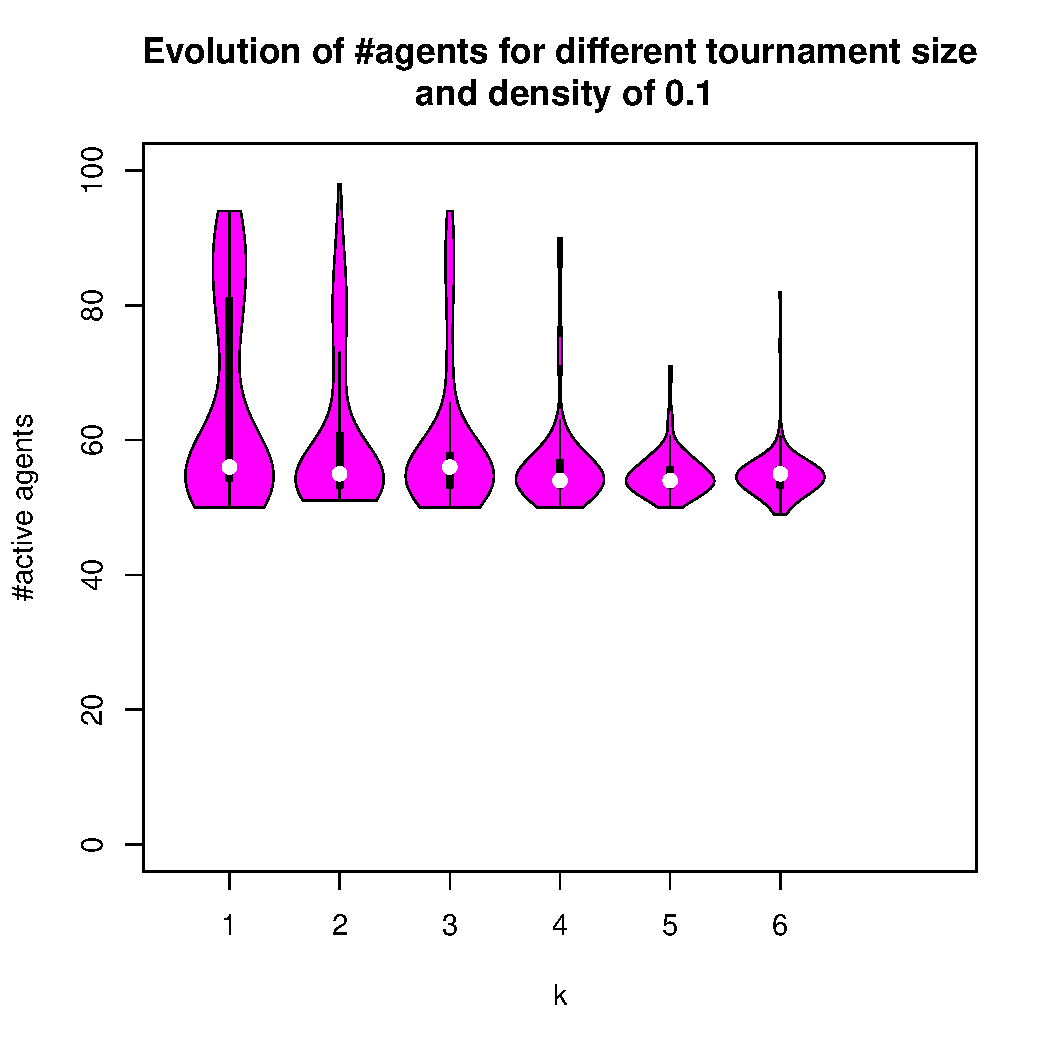
\includegraphics[width=.25\textwidth]{img/100/agentwrtK_D-0100.pdf} &
	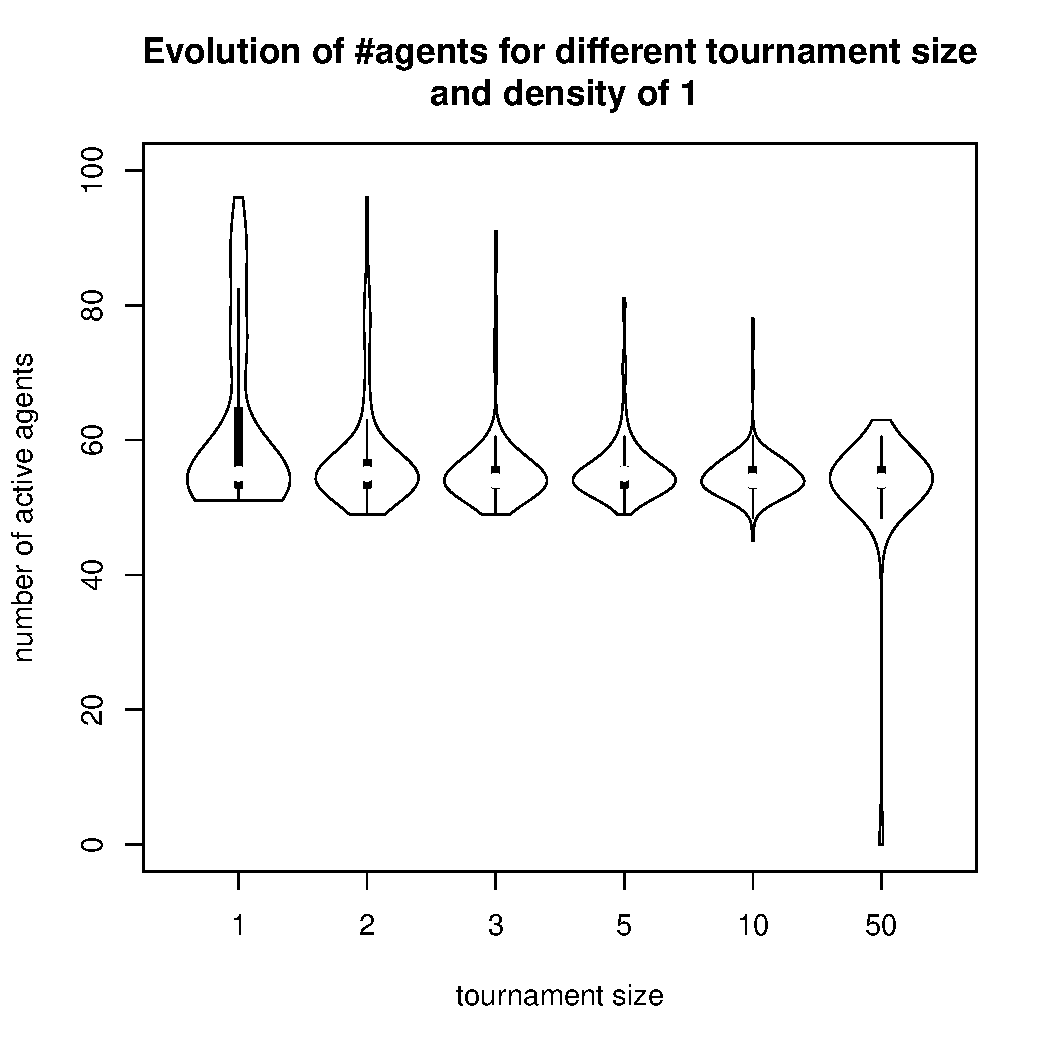
\includegraphics[width=.25\textwidth]{img/100/agentwrtK_D-1000.pdf} \\
	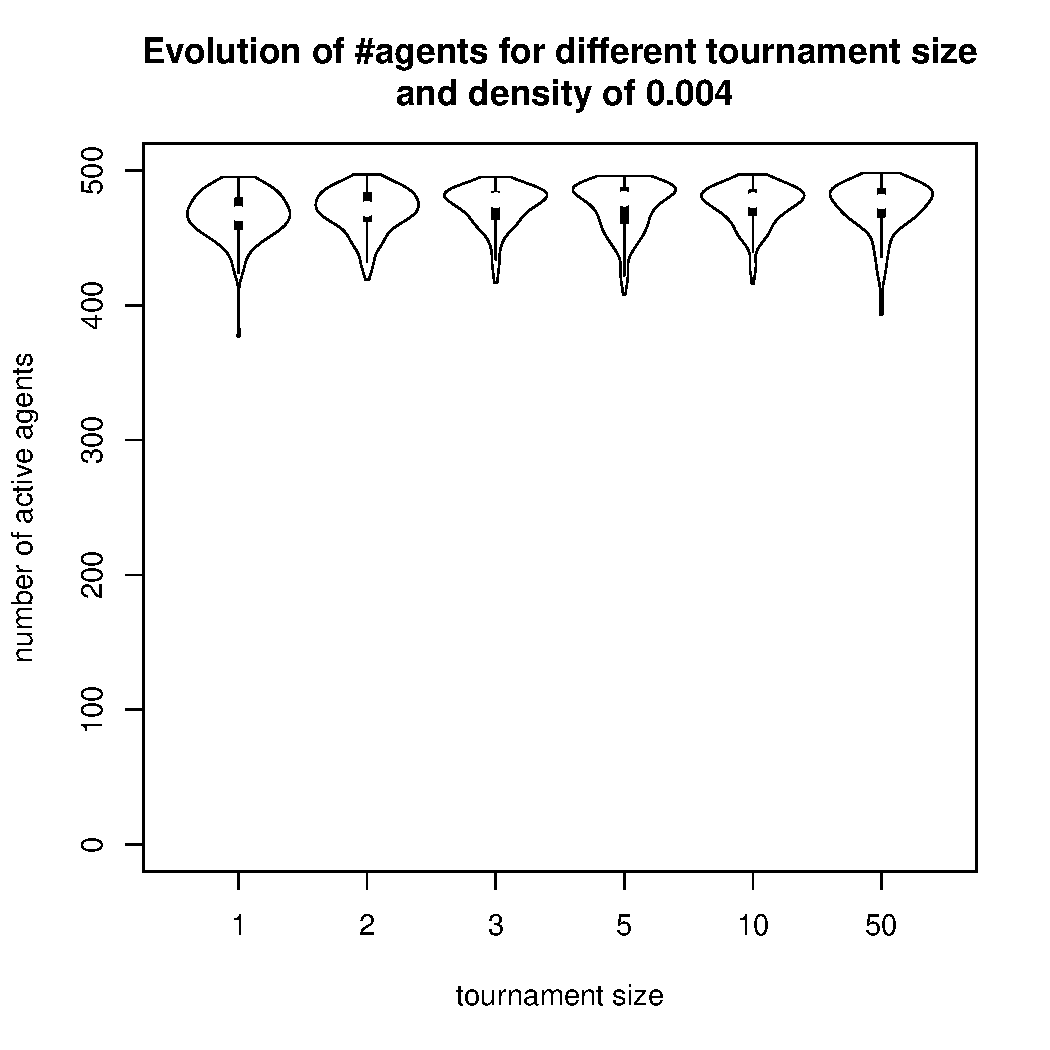
\includegraphics[width=.25\textwidth]{img/500/agentwrtK_D-0004.pdf} &
	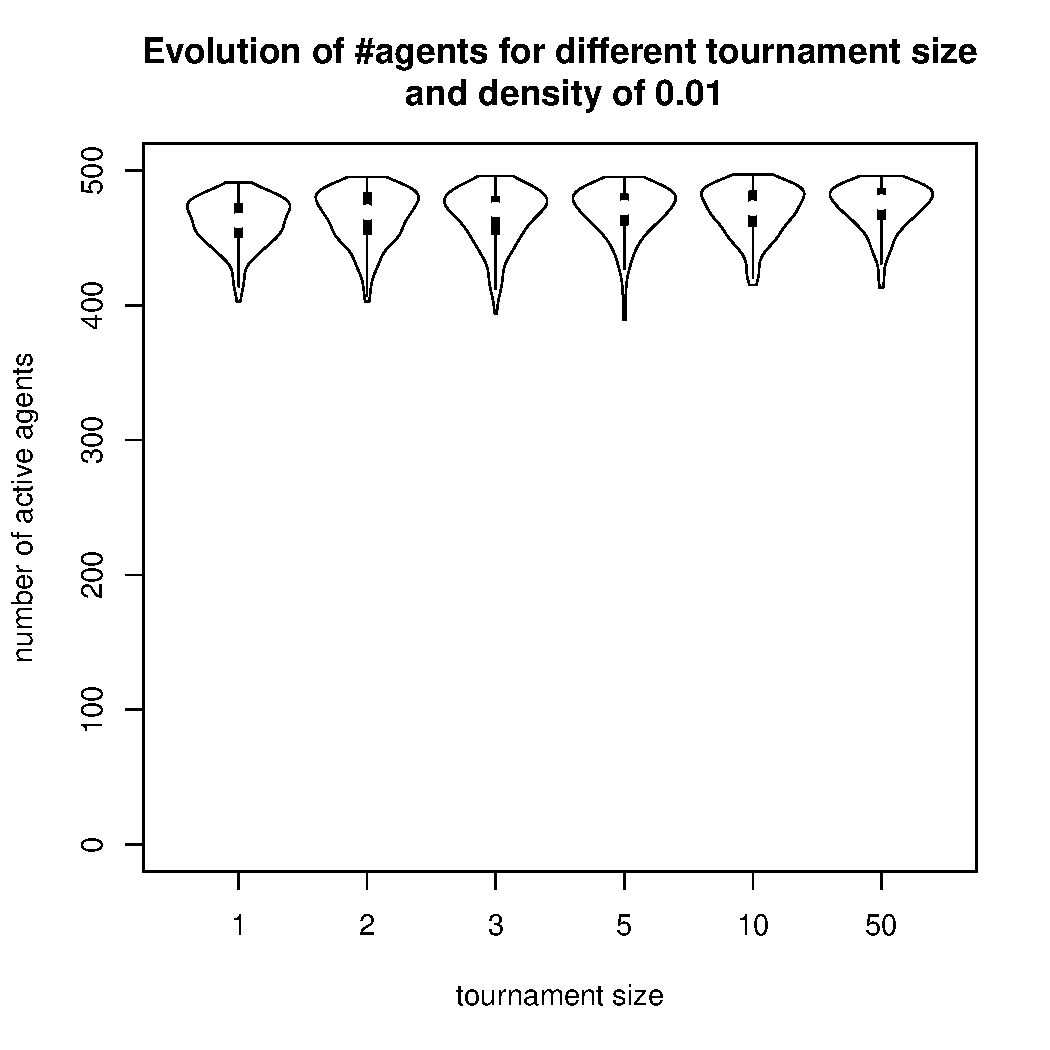
\includegraphics[width=.25\textwidth]{img/500/agentwrtK_D-0010.pdf} &
	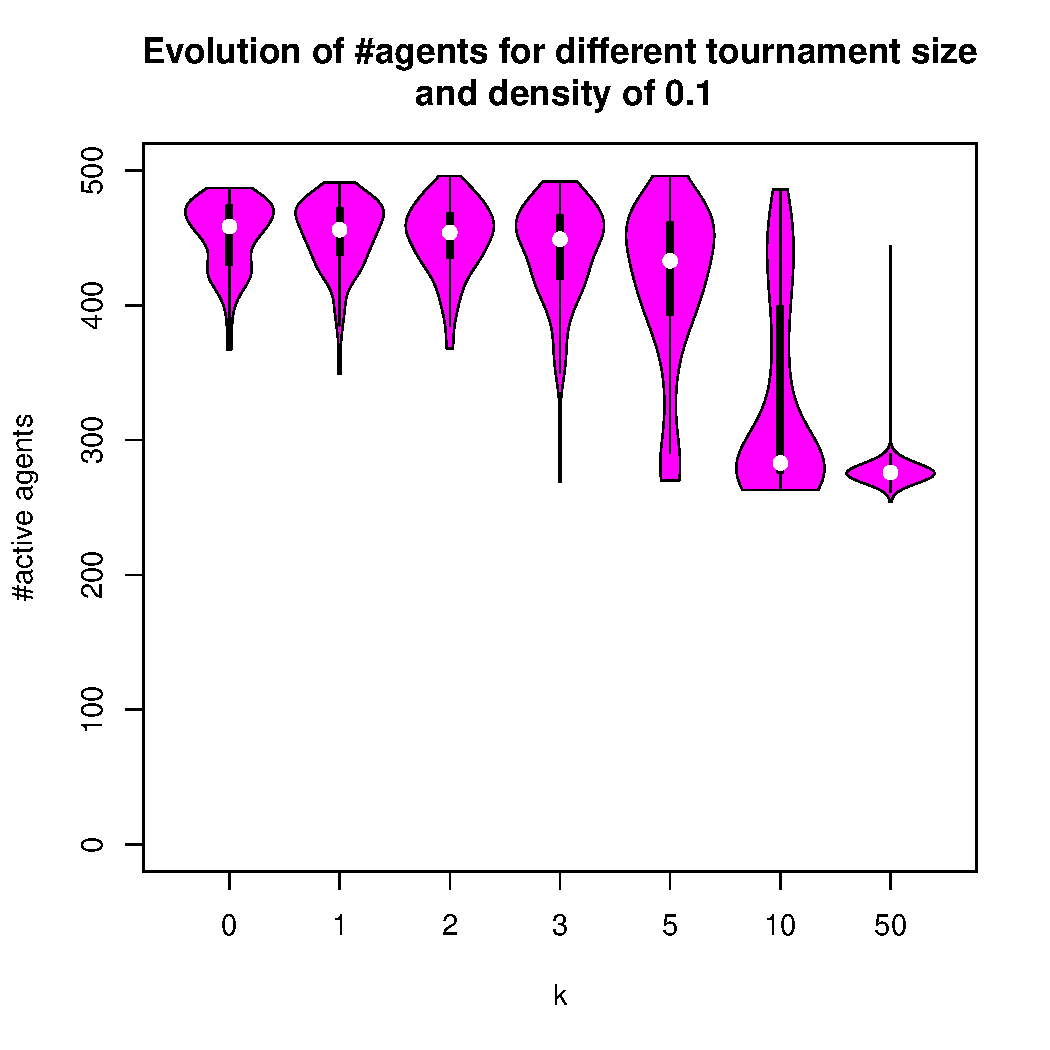
\includegraphics[width=.25\textwidth]{img/500/agentwrtK_D-0100.pdf} &
	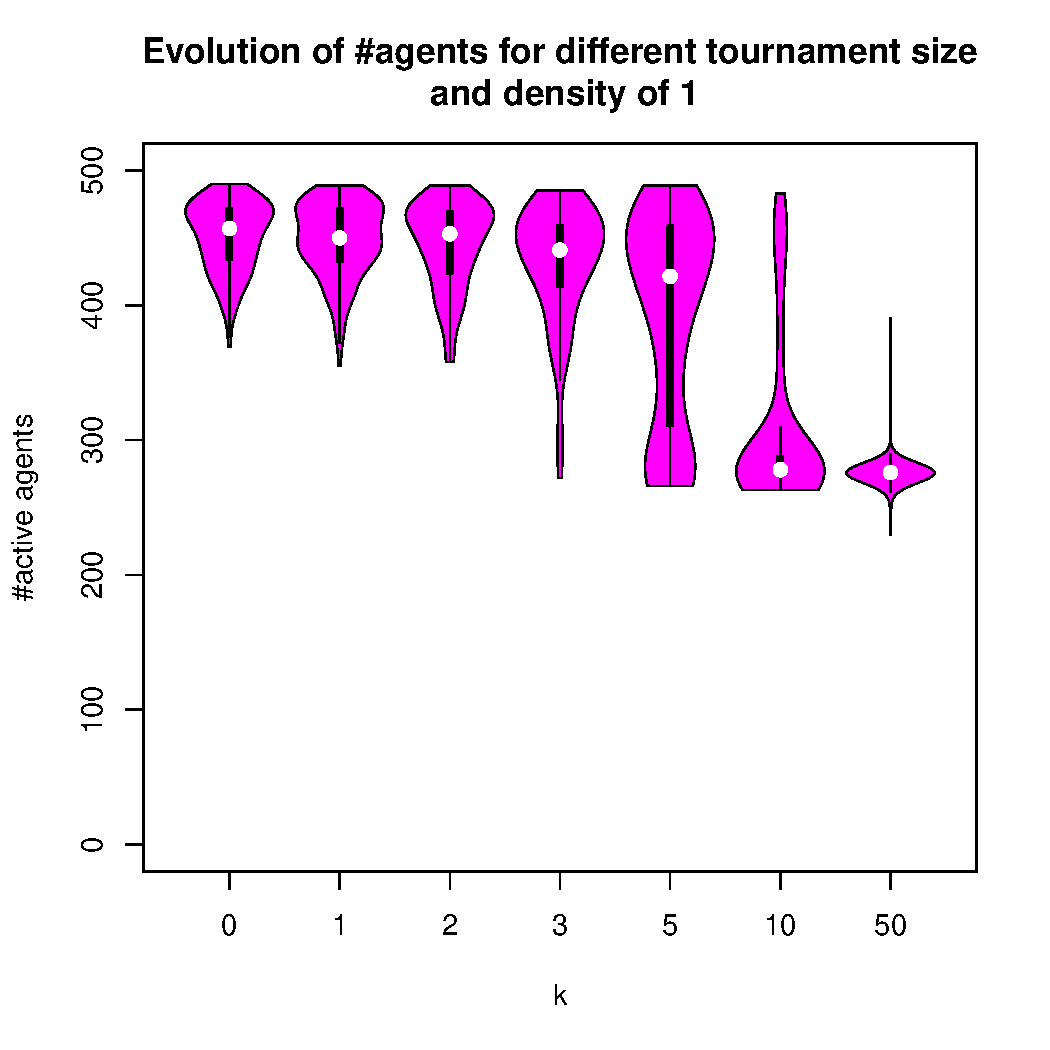
\includegraphics[width=.25\textwidth]{img/500/agentwrtK_D-1000.pdf} \\
    \end{tabular}
    \caption{Number of agent alive at the end of the simulation for different tournament size and differents density. First line show result for simulation with 100 agents, second line for simu with 500 agents }
\end{figure}

\pagebreak

%\section{Resource repartition}
\begin{figure}
    \begin{tabular}[H]{cccl}
	S(50,50) & S(25,75) & S S(90,10)\\
	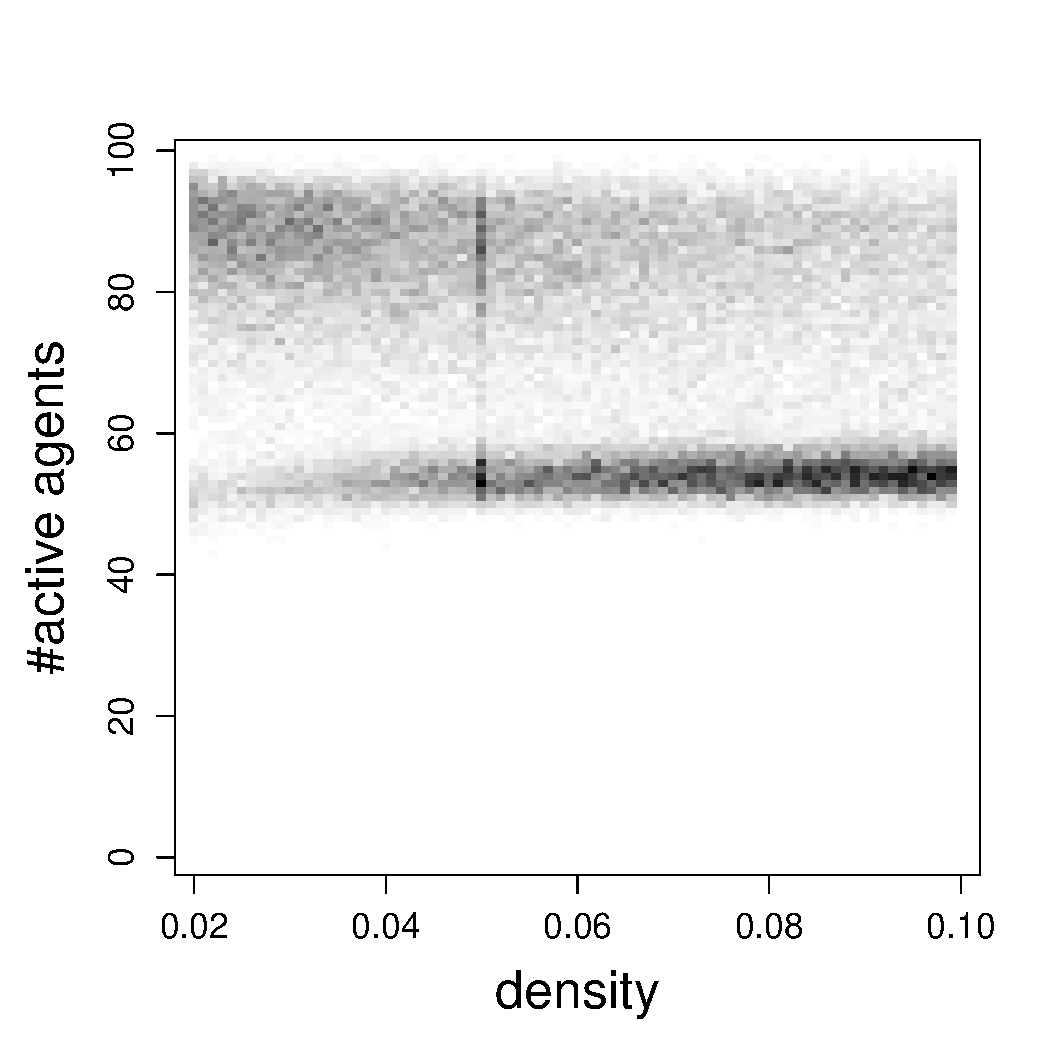
\includegraphics[height=4cm]{img/slice_alive_rep-50.pdf} &
	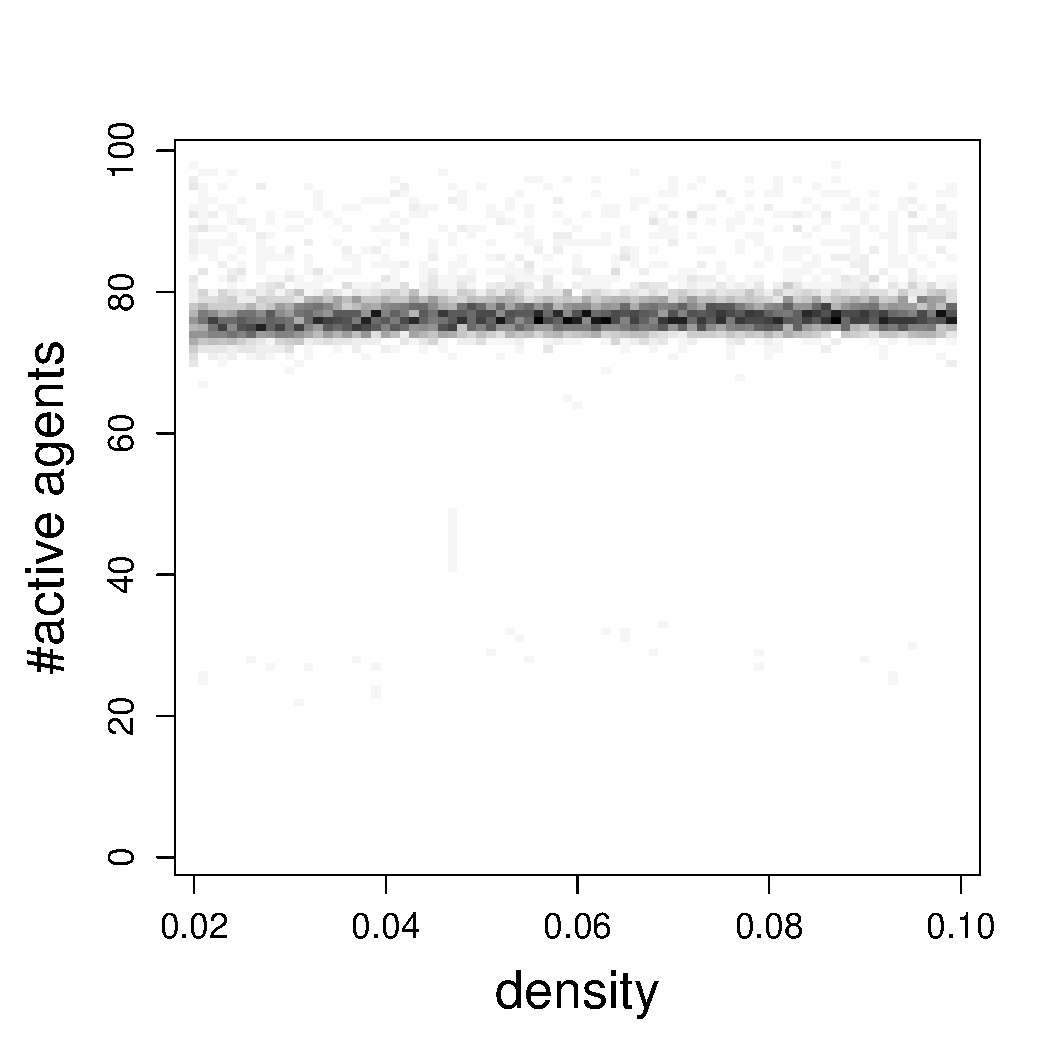
\includegraphics[height=4cm]{img/slice_alive_rep-75.pdf} &
	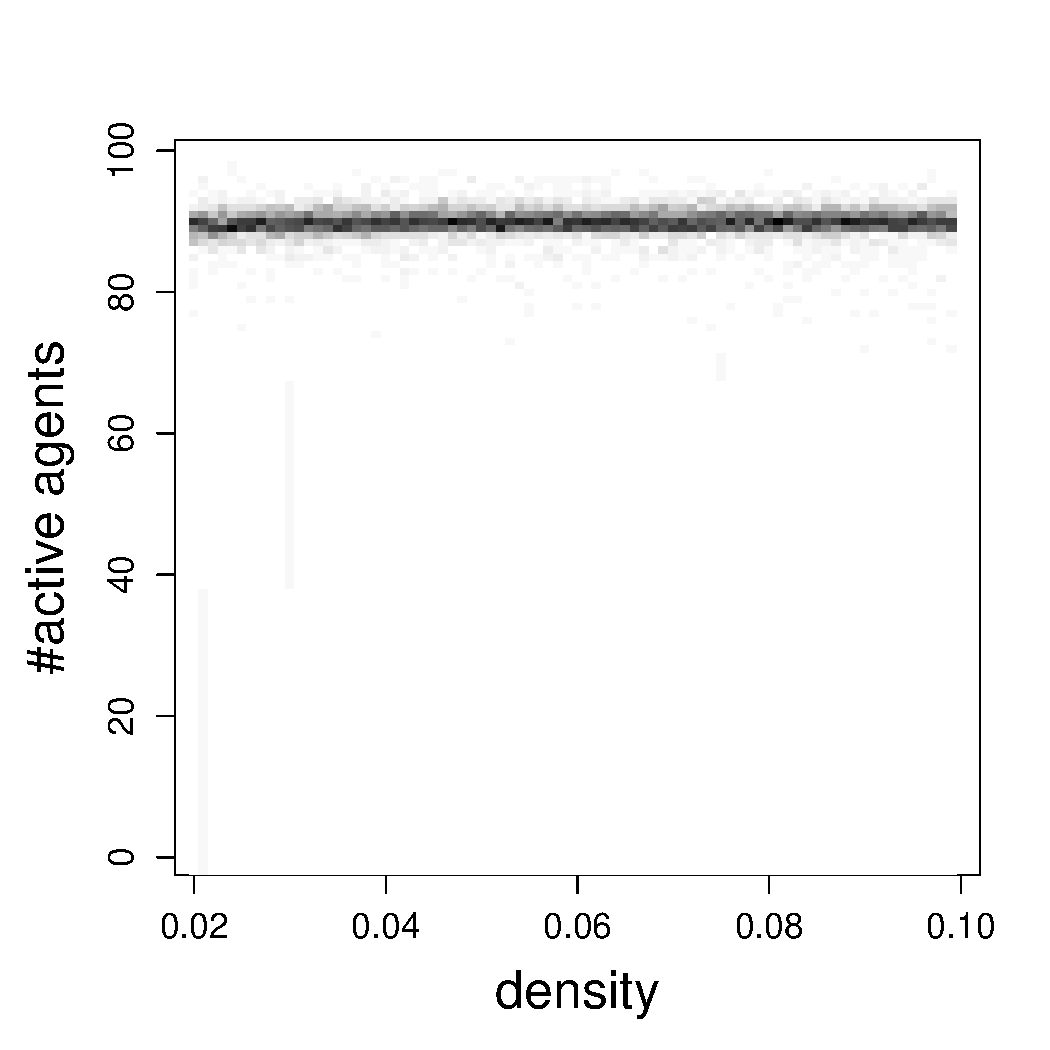
\includegraphics[height=4cm]{img/slice_alive_rep-90.pdf} &
	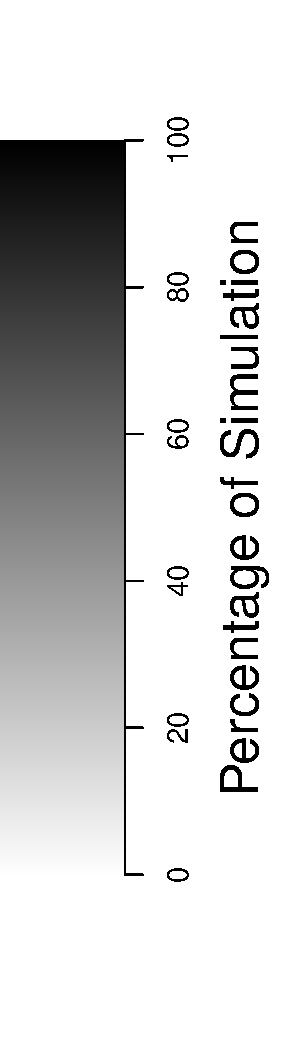
\includegraphics[height=4cm]{img/legNum.pdf} \\
	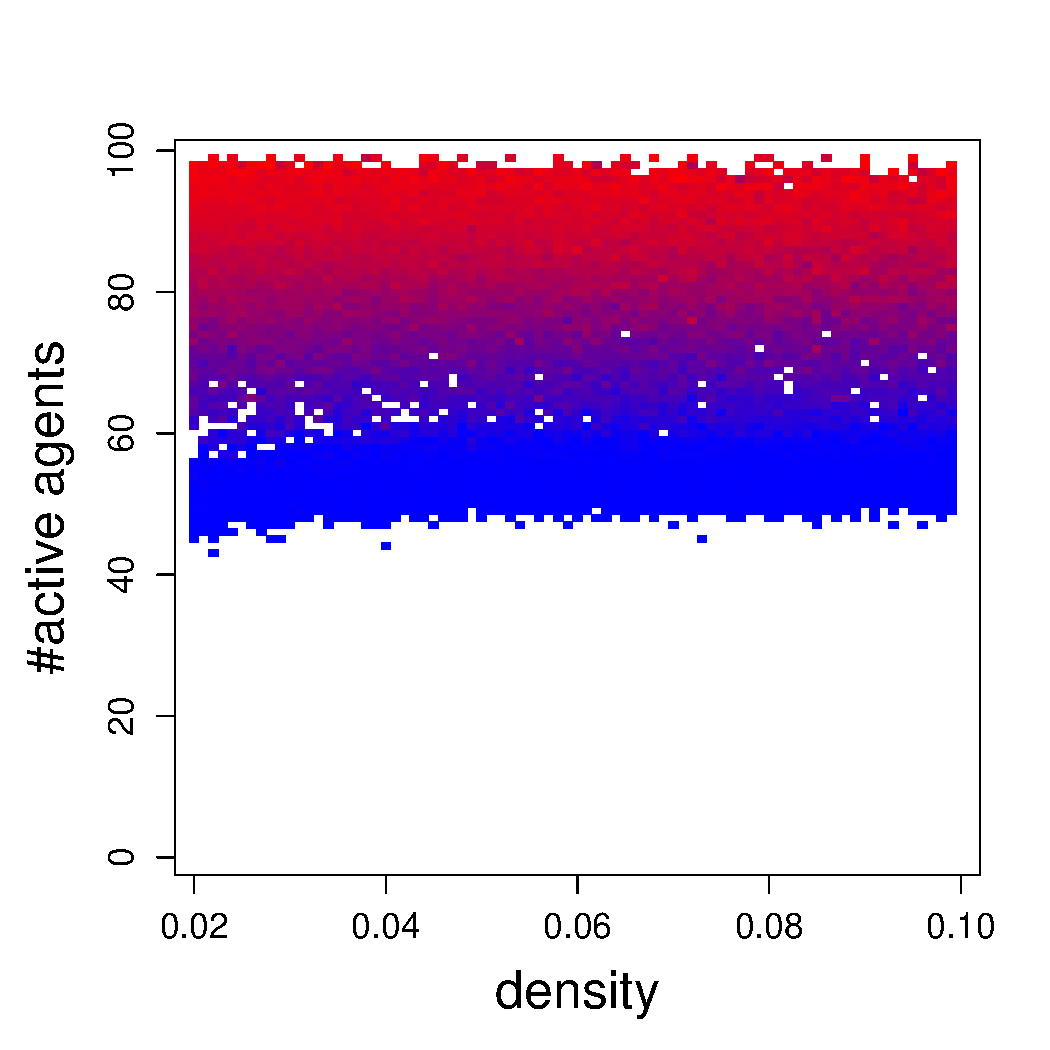
\includegraphics[height=4cm]{img/slice_spec_rep-50.pdf} &
	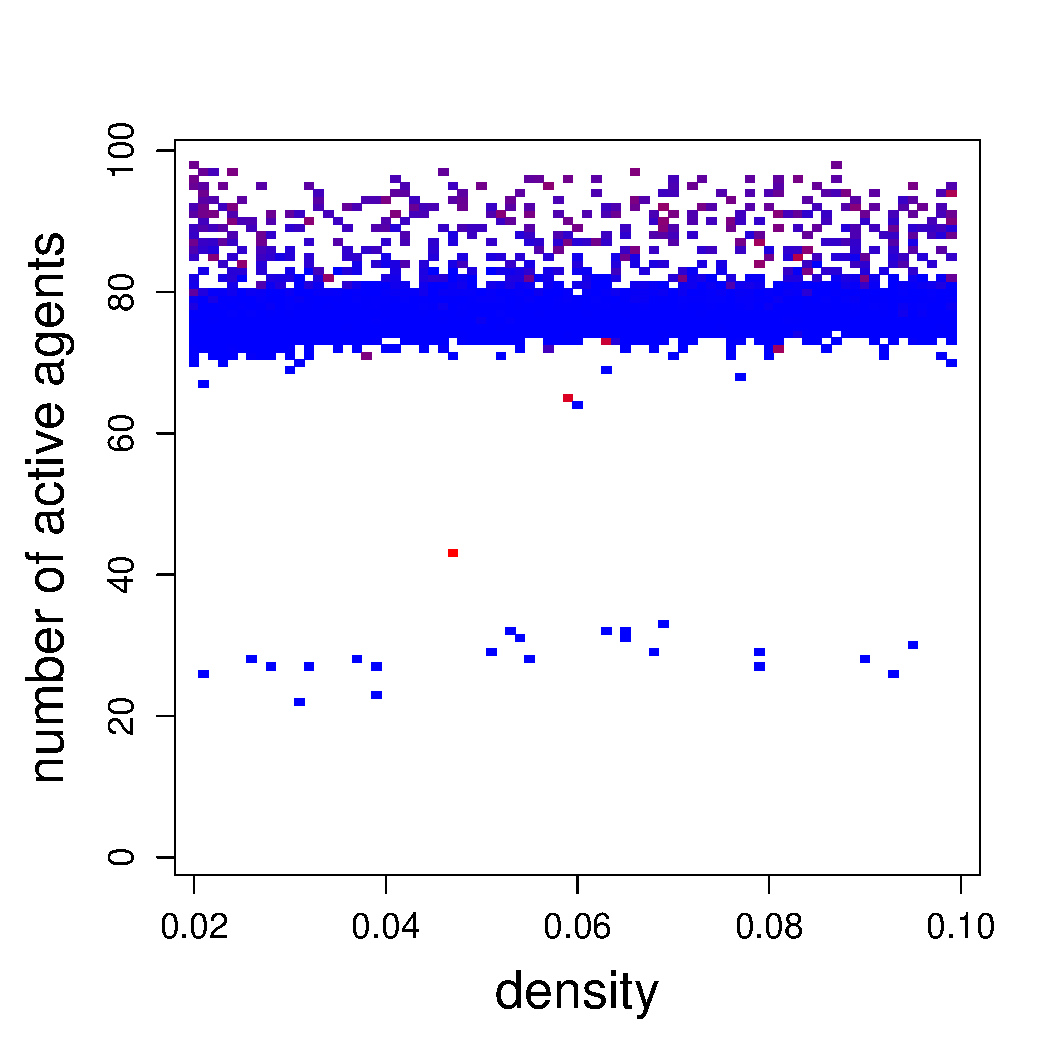
\includegraphics[height=4cm]{img/slice_spec_rep-75.pdf} &
	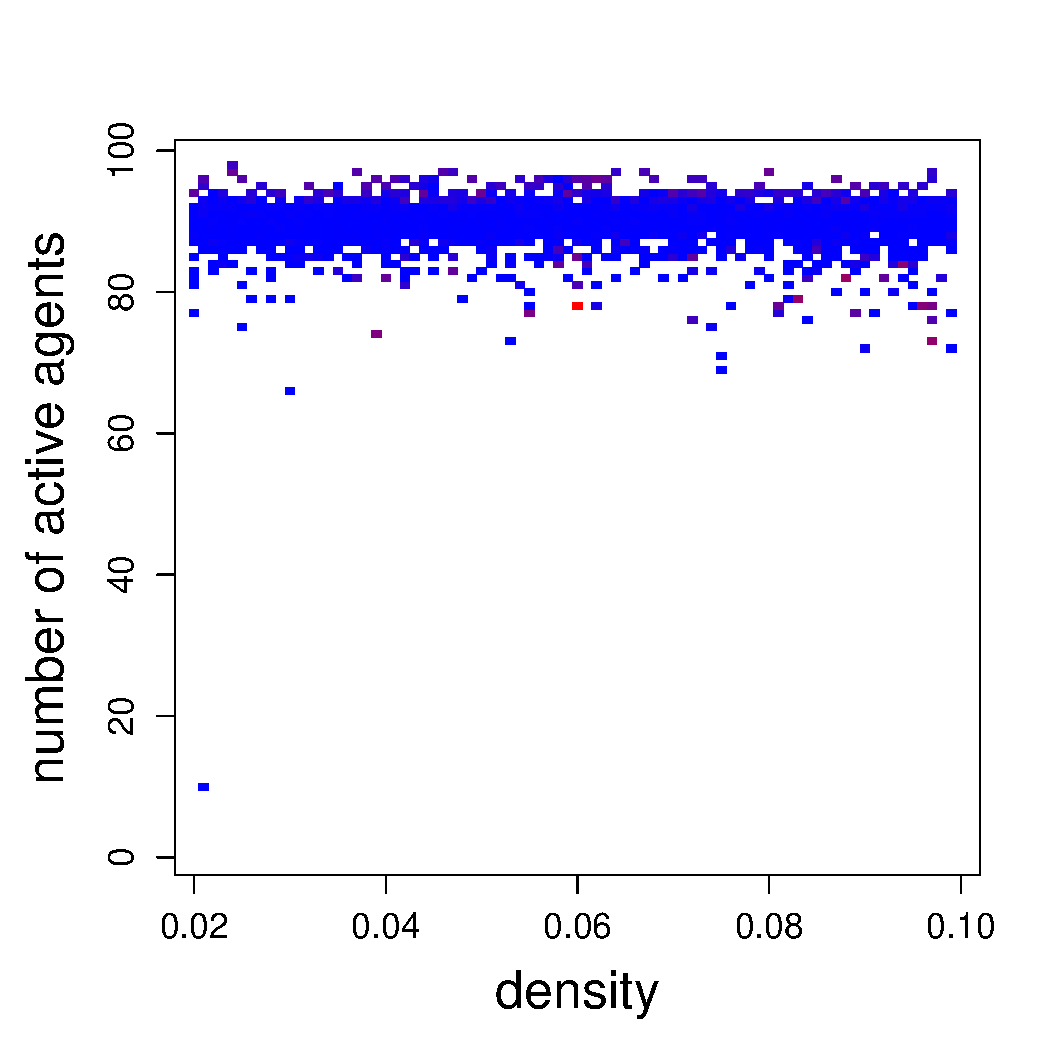
\includegraphics[height=4cm]{img/slice_spec_rep-90.pdf} &
	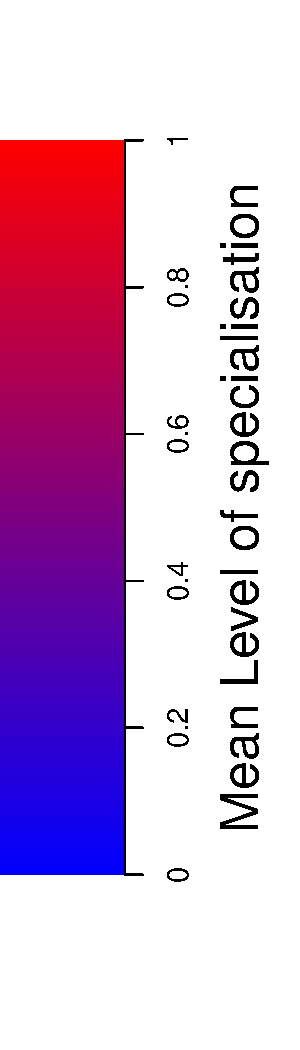
\includegraphics[height=4cm]{img/legLofS.pdf} \\
    \end{tabular}
    \caption{All result for popsize=100. Percentage of Simulation(first line) means: ``the percentage of simulation reaching this number of agents alive at the end of the simulation'',	Mean level of specialisation (2nd line) correspond to the mean between all simulation of : $\frac{min(H(R_1),H(R_2))}{max(H(R_1),H(R_2))}$, \emph{ie} when blue : only one type ; when red:perfect specialisation.
Donc l'idée ici ce serait de mixer les deux lignes, mais ce n'est pas si simple de manipuler les couleurs sur toutes ces dimensions de sorte à ce que ce soit clair et dans sortir une image. Pour l'instant je suis encore entrain de chercher, et je prends toute suggestion.
}
    \label{table:heatmaps}
\end{figure}
\begin{figure}
    \begin{tabular}[H]{ccc}
	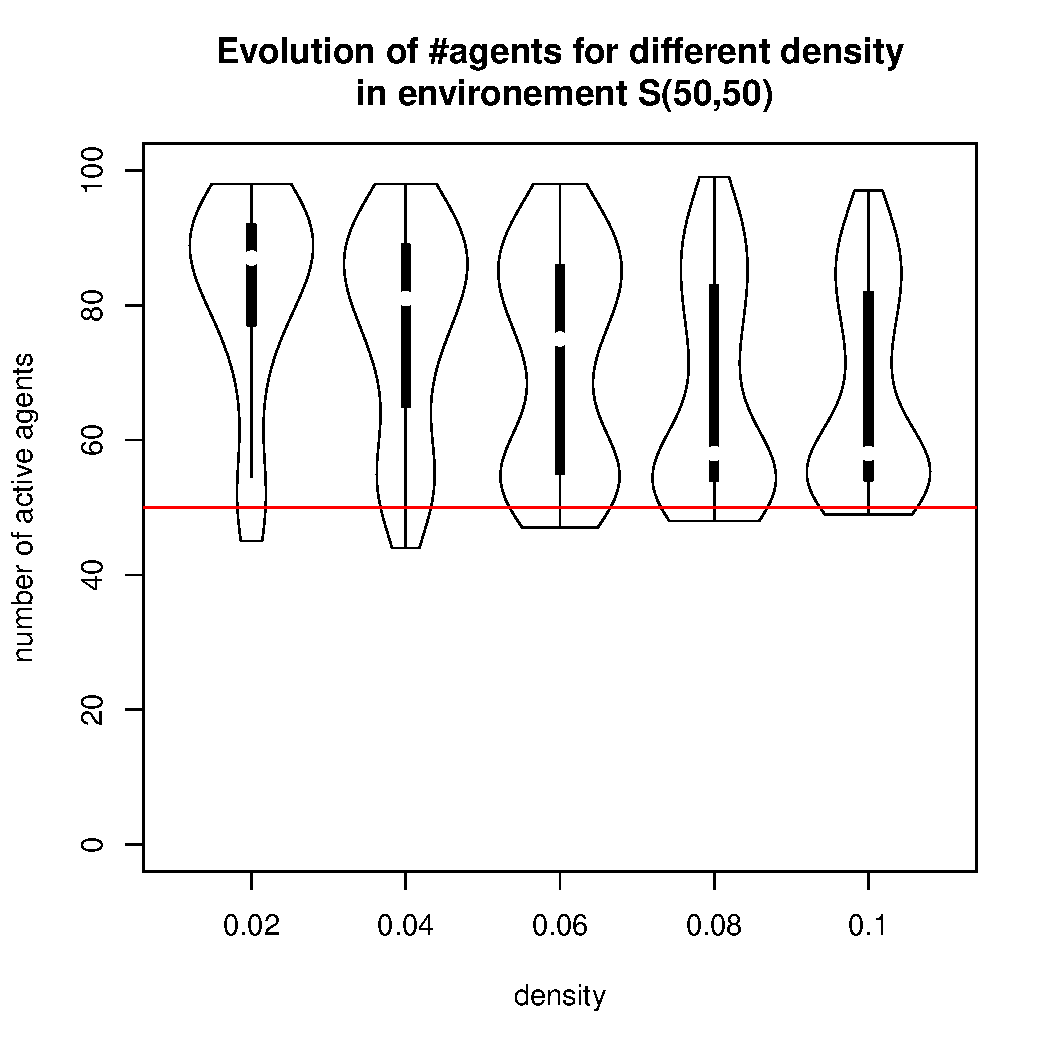
\includegraphics[height=4cm]{img/100/agentwrtD-REP50.pdf} &
	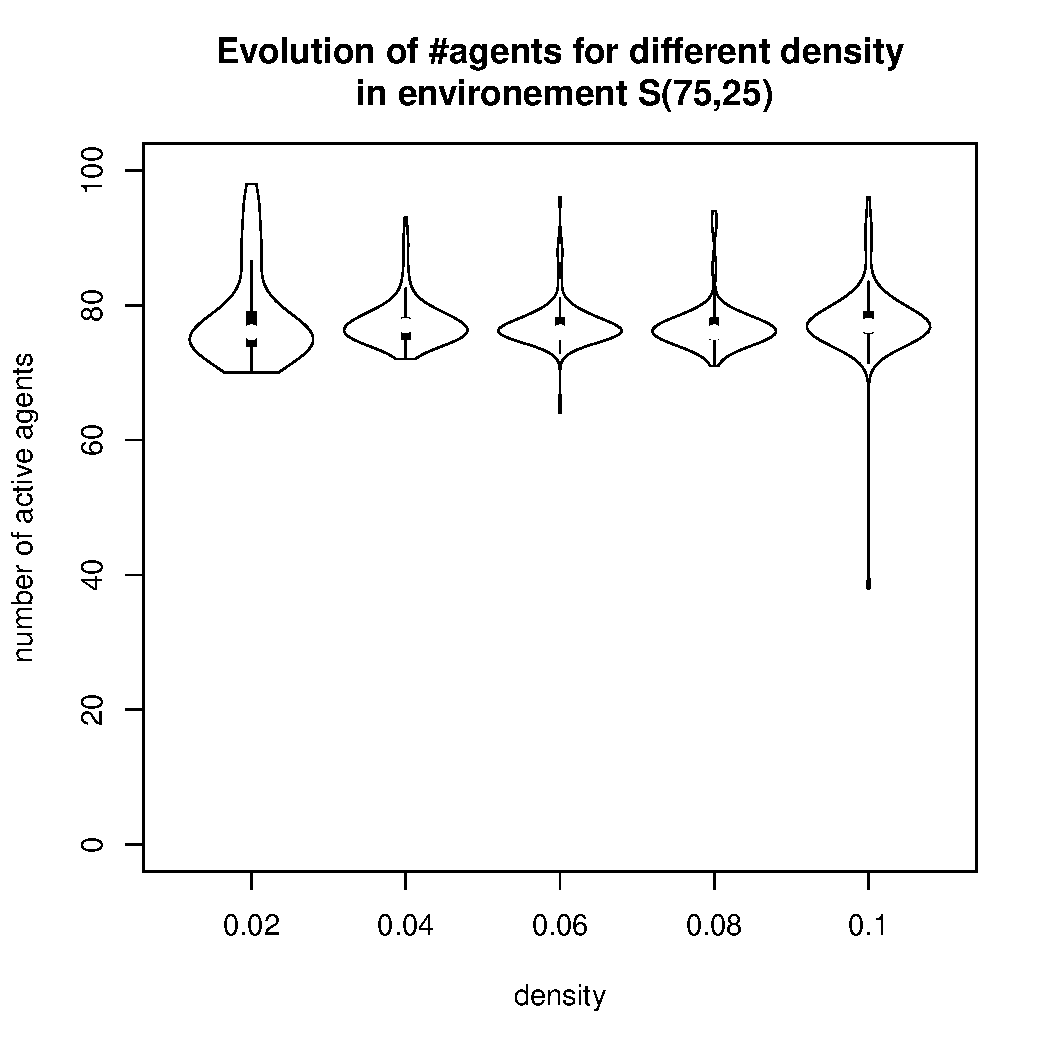
\includegraphics[height=4cm]{img/100/agentwrtD-REP75.pdf} &
	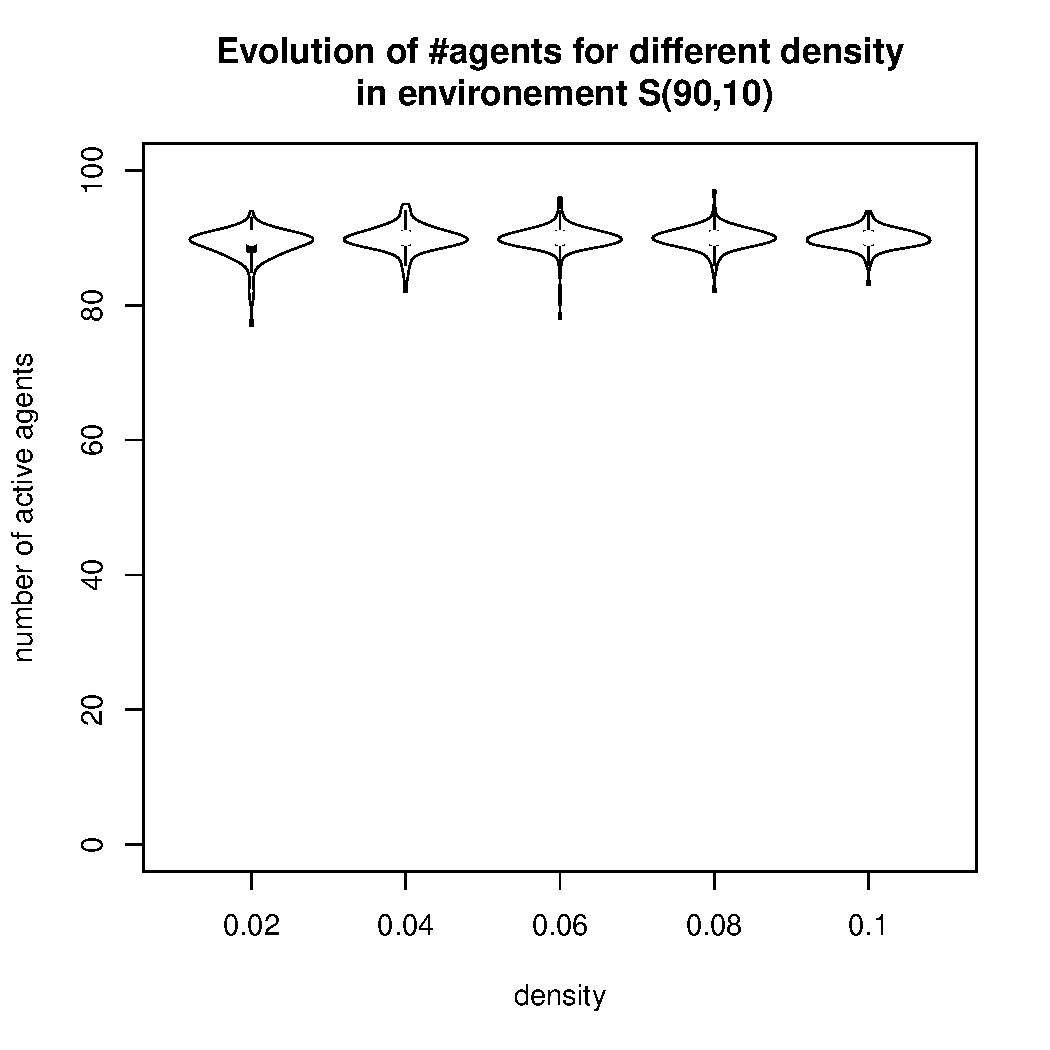
\includegraphics[height=4cm]{img/100/agentwrtD-REP90.pdf} \\
	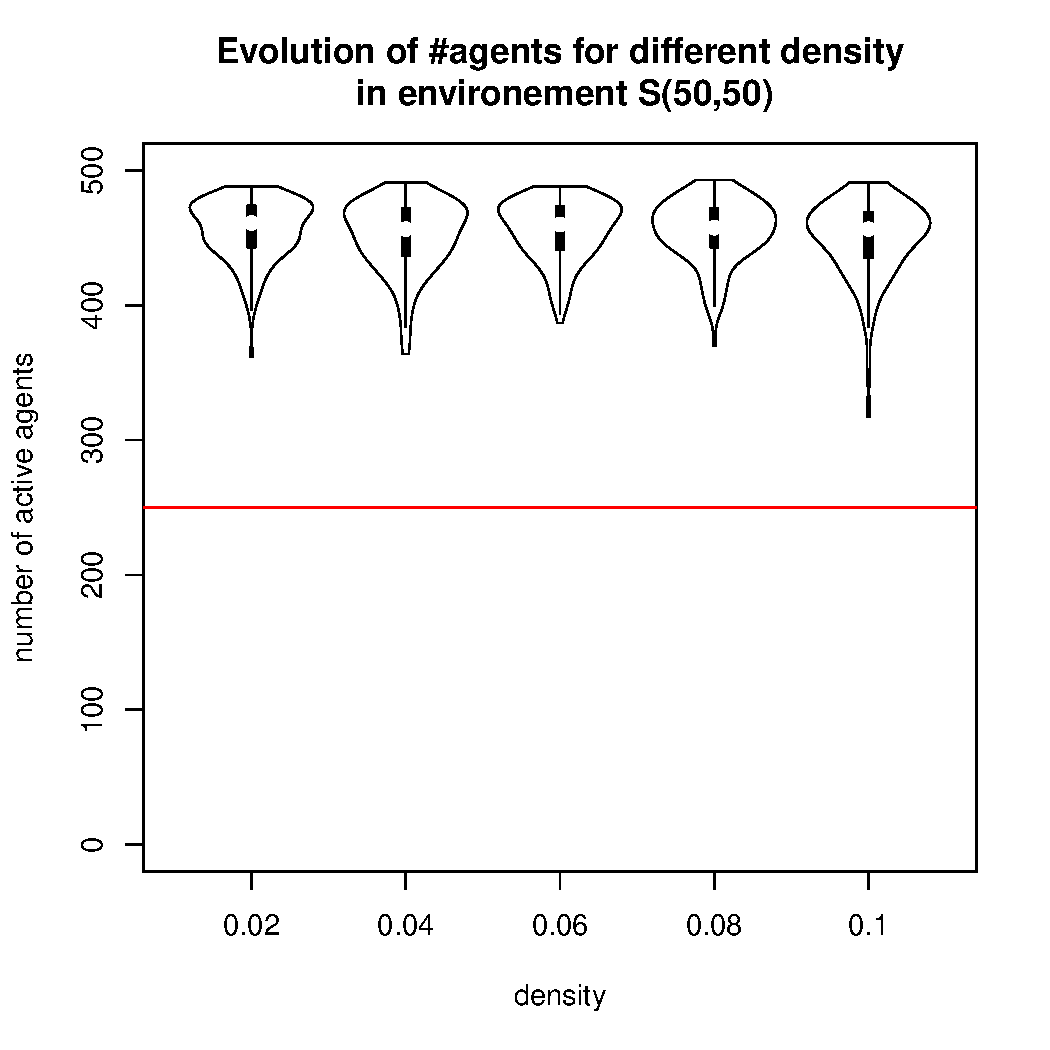
\includegraphics[height=4cm]{img/500/agentwrtD-REP50.pdf} &
	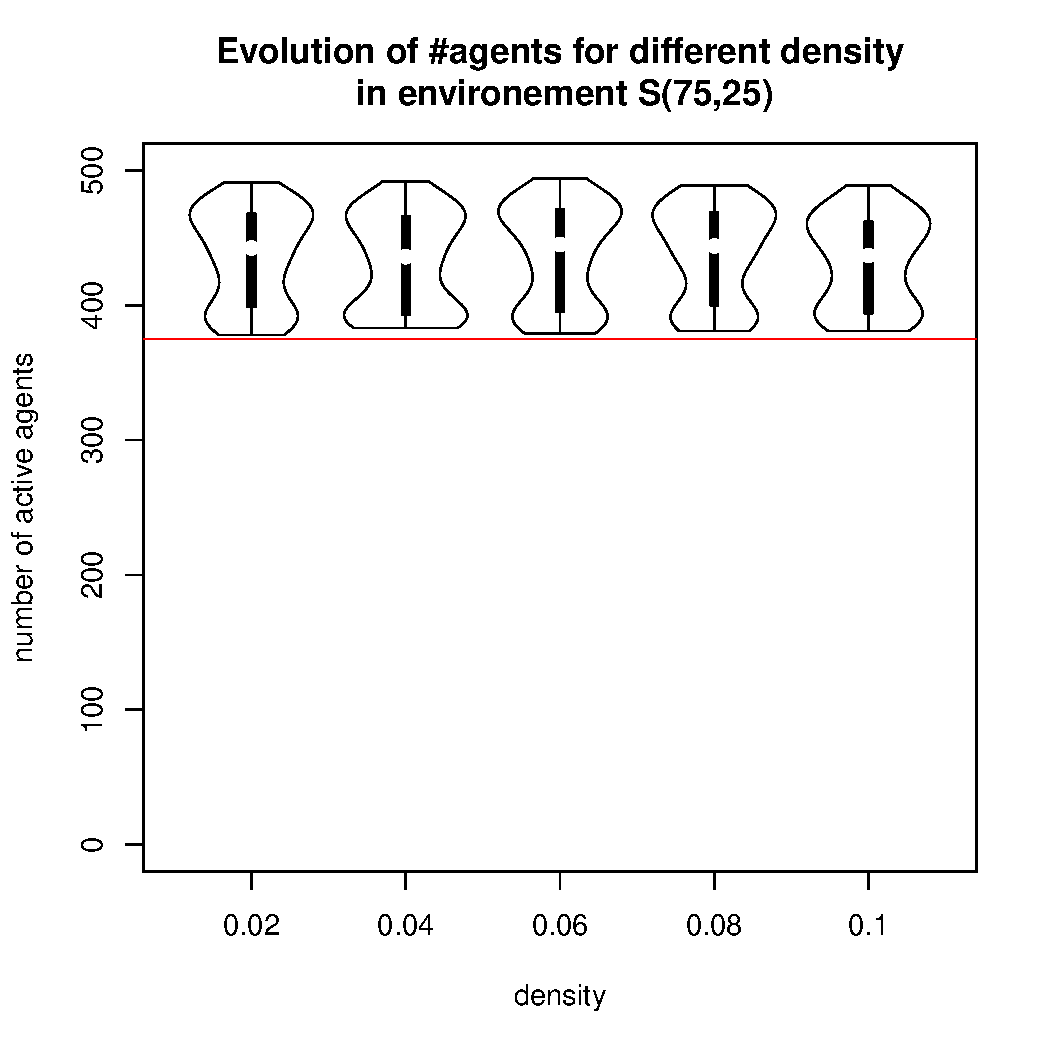
\includegraphics[height=4cm]{img/500/agentwrtD-REP75.pdf} &
	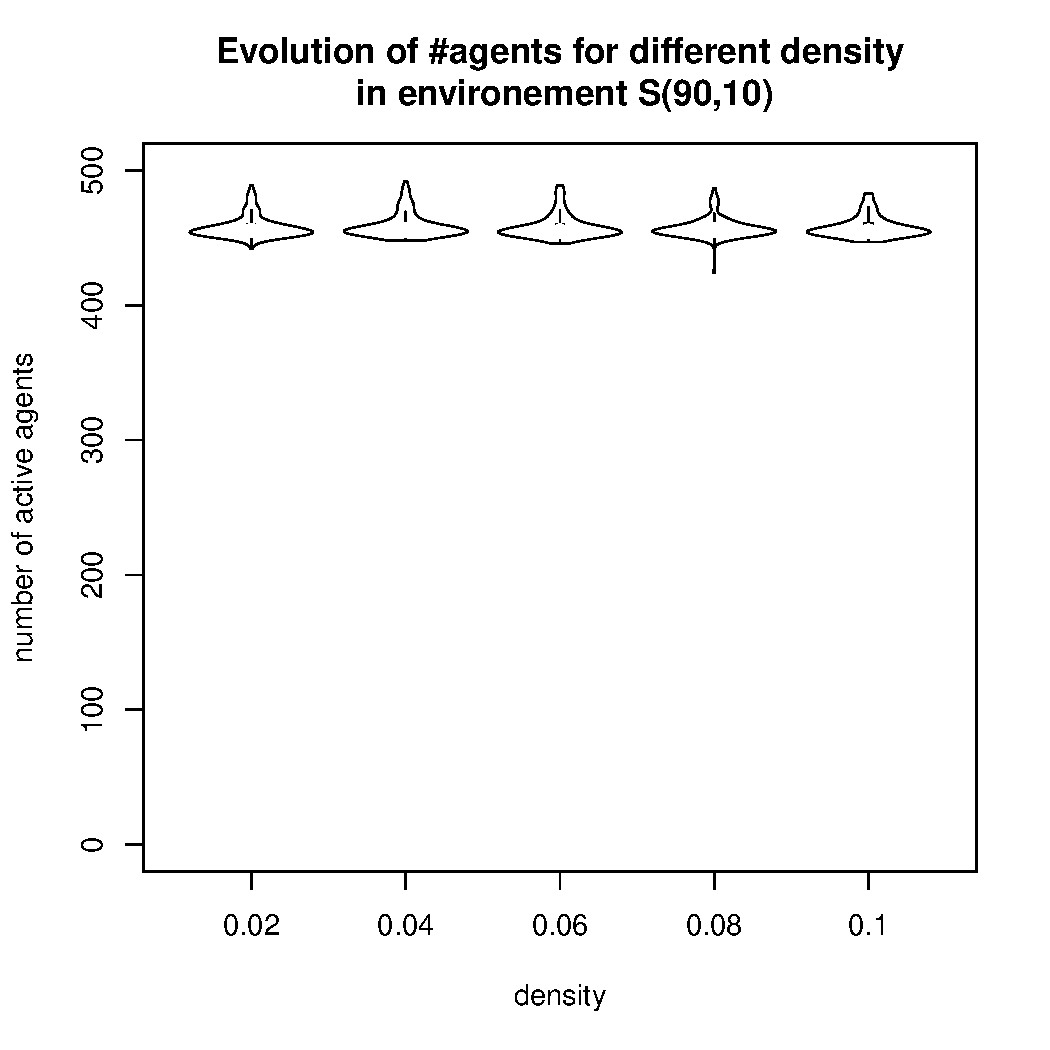
\includegraphics[height=4cm]{img/500/agentwrtD-REP90.pdf} \\
    \end{tabular}
    \caption{Number of agent alive at the end of the simulation for different densities and differents repartition of ressources. Mêmes graphes que la figure precedante mais en les affichant simplement avec des violin plot et pour seulement quelques densités.}
    \label{table:violin}
\end{figure}

\end{document}


